% Estas slides tienen que abrirse con el programa pdfpc que soporta videos embebidos. Para los videos se requiere ubuntu-restricted-extras. El comando es: pdfpc -g slides.pdf

% compress: Encabezado muestra solo la section actual
\documentclass[compress]{beamer}
\mode<presentation>

\usetheme{Copenhagen}
\useoutertheme{taihu}
\useinnertheme{rectangles}

% Itemize configuration
\setbeamertemplate{itemize item}[rectangle]
\setbeamertemplate{itemize subitem}[circle]
\setbeamertemplate{itemize subsubitem}[triangle]

\setbeamertemplate{navigation symbols}{} % Remover símbolos de navegación
\usefonttheme[onlymath]{serif} % Símbolos matemáticos en Serif

\setbeamertemplate{blocks}[rounded] % Block corners rounded
\setbeamercolor{block body}{bg=blue!12,fg=black} % Color of blocks

\usepackage{pdfpc-commands} % pdfpc movie commands
\usepackage[utf8]{inputenc}
\usepackage[spanish]{babel}
\usepackage[binary-units=true]{siunitx} % Para manejar las unidades
\usepackage{multirow}
\usepackage{multimedia}
\usepackage{graphicx}
\usepackage{xcolor}
\usepackage{booktabs} % \toprule

% Elimina la palabra 'Figura' del caption
\usepackage[caption=false]{subfig}
\setbeamertemplate{caption}{\raggedright\insertcaption\par}
\captionsetup[subfigure]{labelformat=empty} % Remover índice del caption de la subfigura

\usepackage{import} % Para el comando import (se usa para pdf_tex)

% Para notas personales en el pdfpc
\usepackage{pdfpcnotes}

%\AtBeginSection[]
%{
%   \begin{frame}
%       \frametitle{Índice}
%       \tableofcontents[currentsection]
%   \end{frame}
%}

\setbeamercovered{transparent}

\usepackage{amsmath}
\usepackage{amssymb}
\usepackage{amsopn}

% math
\renewcommand{\vec}[1]{\boldsymbol{\mathbf{#1}}}
\newcommand{\norm}[1]{\left\lVert#1\right\rVert}

% Declare arg max and arg min functionss
\DeclareMathOperator*{\argmax}{arg\,max}
\DeclareMathOperator*{\argmin}{arg\,min}

% Homogeneous decoration function
\newcommand{\homo}[1]{\dot{#1}}

% Declare projection as math function
\DeclareMathOperator{\proj}{proj}
\DeclareMathOperator{\disp}{disp}
\newcommand{\worldCoordSystem}{\mathrm{w}}
\newcommand{\cameraCoordSystem}{\mathrm{c}}
\newcommand{\point}{\vec{x}}
\newcommand{\worldPoint}{\point^{\mathrm{w}}}
\newcommand{\homoWorldPoint}{\homo{\point}^{\mathrm{w}}}
\newcommand{\cameraPoint}{\point^{\mathrm{c}}}
\newcommand{\hatCameraPoint}{\hat{\point}^{\mathrm{c}}}
\newcommand{\homoCameraPoint}{\homo{\point}^{\mathrm{c}}}
\newcommand{\measurement}{\vec{z}}
\newcommand{\prediction}{\hat{\vec{z}}}
\newcommand{\imagePoint}{\vec{u}}
\newcommand{\seMatrix}{\vec{E}}
\newcommand{\rotation}{\vec{R}}
\newcommand{\translation}{\vec{t}}
\newcommand{\intrinsicMatrix}{\vec{K}}
\newcommand{\principalPoint}{\vec{c}}
\newcommand{\reprojectionError}{u}
\newcommand{\projectionMatrix}{\vec{P}}
\newcommand{\cameraCenter}{\vec{o}}


% Dense Map
\newcommand{\current}{\mathrm{current}}
\newcommand{\previous}{\mathrm{previous}}
\newcommand{\fusion}{\mathrm{fusion}}
\newcommand{\inverseDepth}{\rho}
\newcommand{\plane}{\boldsymbol{\pi}}
\newcommand{\reference}{ref}


% scaled operators and letters to fancy view
\newcommand{\sminus}{\scalebox{0.5}[1.0]{$-$}}
\newcommand{\splus}{\scalebox{0.6}[0.6]{$+$}}
\newcommand{\curr}{c}
\newcommand{\sind}[1]{\scalebox{0.6}[0.6]{$#1$}}
\newcommand{\ind}[1]{\scalebox{0.7}[0.7]{$#1$}}

\newcommand{\keyframe}{\vec{K}}
\newcommand{\pointCloud}{\mathcal P}
\newcommand{\groundTruth}[1]{{#1}^{*}}

\newcommand{\update}[1]{\hat{#1}}

\newcommand{\position}{\vec{p}}
\newcommand{\map}{M}

\newcommand{\baseline}{b}
\newcommand{\focalDistance}{f}
\newcommand{\disparityMap}{\mathcal D}
\newcommand{\camera}{c}
\newcommand{\ray}{n}


\setbeamerfont{normal text}{size*={10}{10}}
\AtBeginDocument{\usebeamerfont{normal text}}

\title{Mapeo denso online sobre sistemas SLAM basados en visión estéreo}
\author{Ariel D'Alessandro}
\institute{Director: Taihú Pire. Co-Director: Rodrigo Baravalle. \\ \vspace{0.5cm} Tesina de Grado \\ Licenciatura en Ciencias de la Computación \\ FCEIA - UNR}
\titlegraphic{
\includegraphics[width=0.14\textwidth]{images/logo-unr.png}}
\date{\scriptsize{22 de diciembre de 2017}}

\begin{document}

\frame{
	\titlepage
	\pnote{
		Soy Ariel y esta es mi tesina.\\
		Agradecer jurado y dcc: Ana, Pablo G., Pablo Pilotti, Juan Carlos Gómez, Claudia Deco, Directores.\\
	}
}


% Frame ---------------------------------------------------------------------
\begin{frame}
	\frametitle{Estructura de la presentación}
	\tableofcontents
	
	\pnote{
		Aportes 2,3,4.\\
	}
\end{frame}


\section{Introducción}


\subsection{Robótica móvil}


\begin{frame}
	\frametitle{Robots móviles}
	\begin{figure}[!h]
		\centering
		\subfloat[] 
		{
			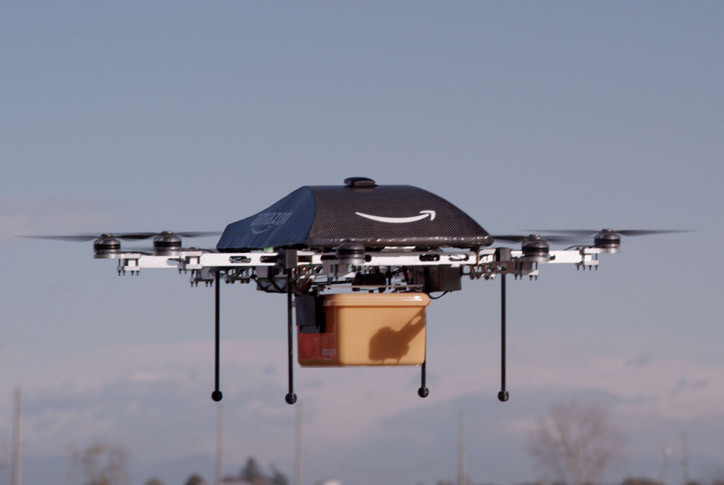
\includegraphics[width=0.33\columnwidth]{./images/introduction/drone.jpg}
		}
		\subfloat[] 
		{
			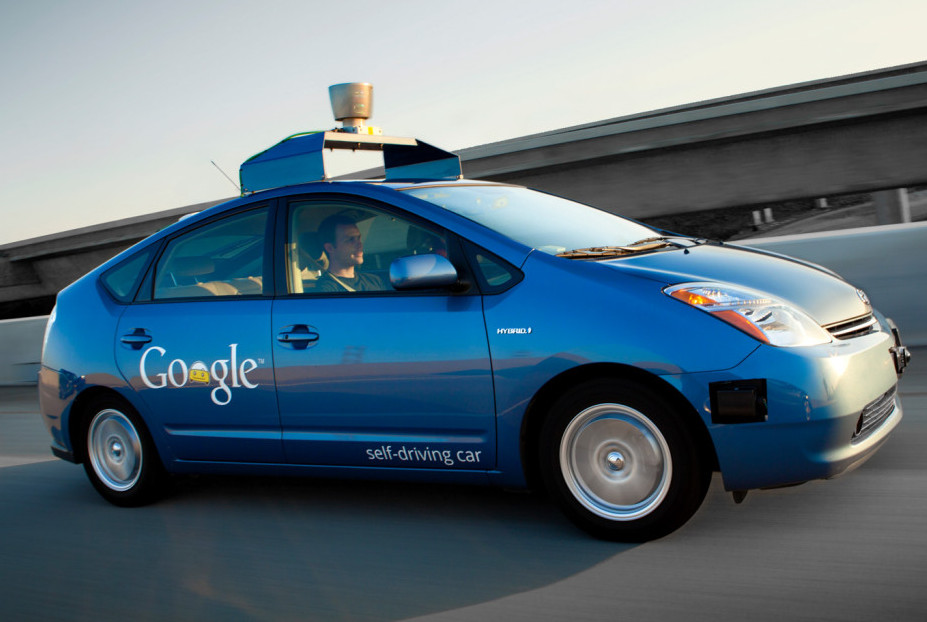
\includegraphics[width=0.33\columnwidth]{./images/introduction/GoogleCar.jpg}
		}
		\subfloat[] 
		{
			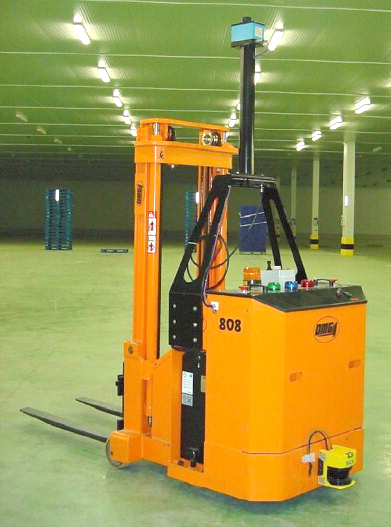
\includegraphics[width=0.16\columnwidth]{./images/introduction/industrial_robot.png}
		}\\
		\subfloat[] 
		{
			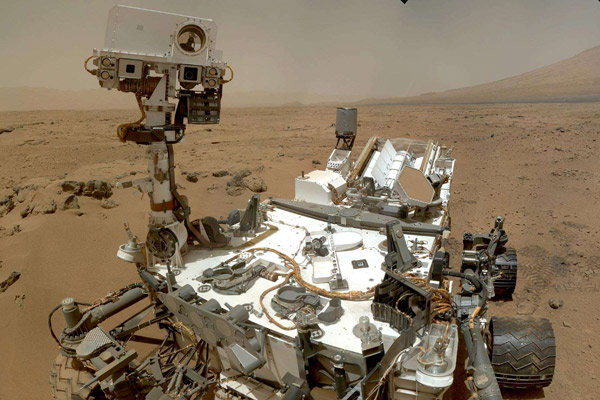
\includegraphics[width=0.33\columnwidth]{./images/introduction/curiosity.png}
		}
		\subfloat[] 
		{
			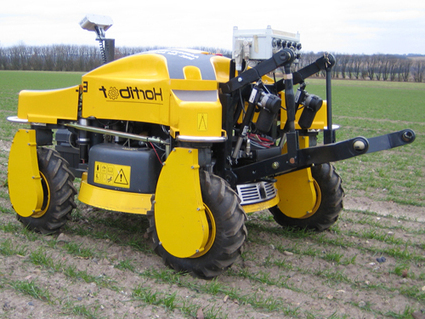
\includegraphics[width=0.33\columnwidth]{./images/introduction/hortibot.png}
		}
		\subfloat[]
		{
			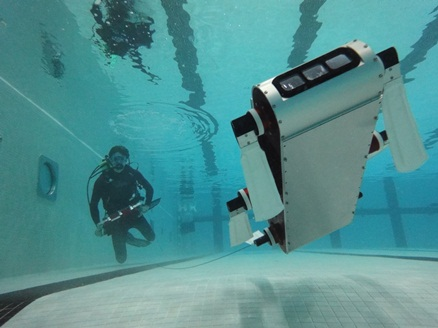
\includegraphics[width=0.33\columnwidth]{./images/introduction/aqua2.png}
		}		 
	\end{figure}
\end{frame}


\begin{frame}
	\frametitle{Navegación autónoma}
	\begin{block}{}
		La navegación autónoma puede definirse a grandes rasgos como la capacidad de moverse de forma segura a lo largo de una trayectoria entre un punto de inicio y uno final [1].
	\end{block}
	\vspace{5mm}
	\begin{columns}
		\column{0.4\textwidth}
		\hspace{13pt}Pregunta:
		\begin{enumerate}
			\visible<2-7>{ \item[-] ¿Dónde estoy?}
			\visible<4-7>{\item[-] ¿Por dónde estoy yendo?}
			\visible<6-7>{\item[-] ¿Cómo llego hasta allí?}
		\end{enumerate}
		\column{0.6\textwidth}
		Respuesta:
		\begin{enumerate}[$\rightarrow$]
			\visible<3-7>{ \item  Cálculo de la posición (Localization)}
			\visible<5-7>{ \item  Representación del entorno (Mapping)}
			\visible<7-7>{\item  Planeamiento de movimiento (Motion planning)}
		\end{enumerate}
	\end{columns}
	\only<4>{}
	\vfill
	\begin{tiny}
		[1] J. J. Leonard - et al., ``Mobile robot localization by ...,'' IEEE Transactions on Robotics and Automation, 2002.
	\end{tiny}
\end{frame}


\subsection{SLAM}


% Frame ---------------------------------------------------------------------
\begin{frame}
	\frametitle{SLAM - Simultaneous Localisation and Mapping}

	\begin{itemize}
        \item Sensores permiten detectar marcas naturales (\textbf{landmarks})
        \begin{itemize}
            \item El robot determina su posición y orientación en base a estas.
            \item Construye incrementalmente un mapa del entorno, ubicando estas marcas en el mismo.
        \end{itemize}
    \end{itemize}

	\vspace{-1em}
	\begin{figure}[!htb]
		\centering
		\subfloat[]{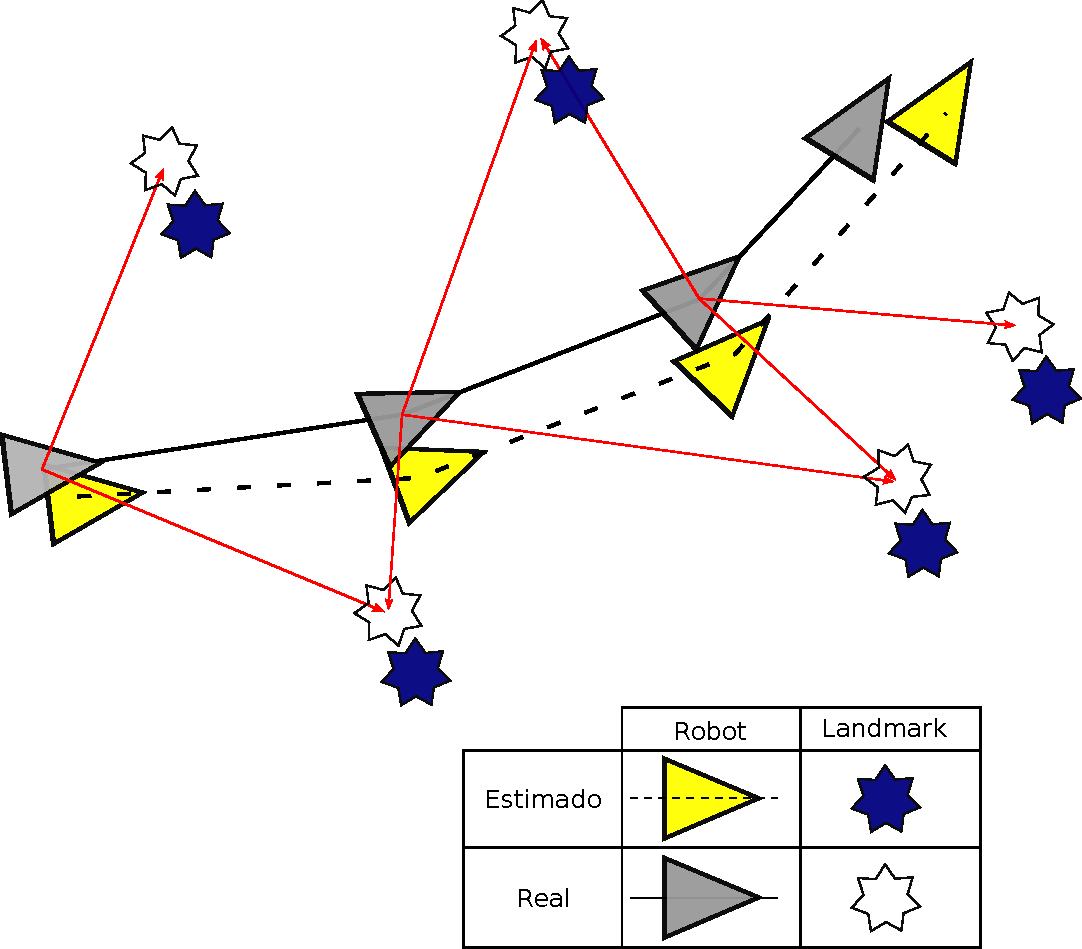
\includegraphics[width=0.6\columnwidth]{./introduction/slam-landmarks.pdf}}
		\hfill
	\end{figure}

\end{frame}


\begin{frame}
	\frametitle{Algunos de los sensores más utilizados}	
	\pnote{
		Telemetro - IR - GPS - IMU - encoders\\
		Sonar - Zed camera - Bumper - Laser\\
	}
	
	\begin{figure}[!h]
		\centering
		\subfloat[] 
		{
			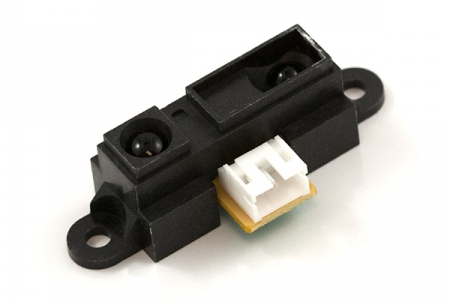
\includegraphics[width=0.225\columnwidth]{images/introduction/telemetro.png}
		}
		\subfloat[] 
		{
			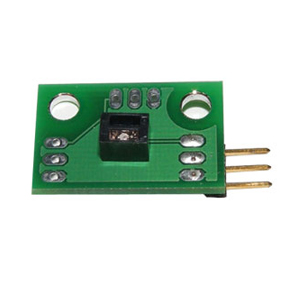
\includegraphics[width=0.15\columnwidth]{images/introduction/ir_sensor.png}
		}
		\subfloat[] 
		{
			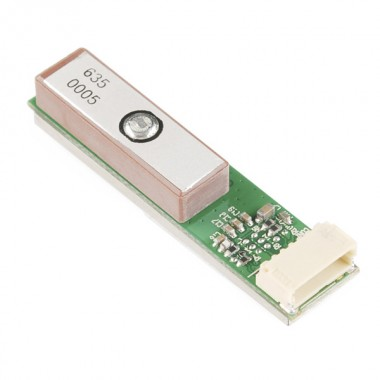
\includegraphics[width=0.18\columnwidth]{images/introduction/gps.jpg}
		}
		\subfloat[] 
		{
			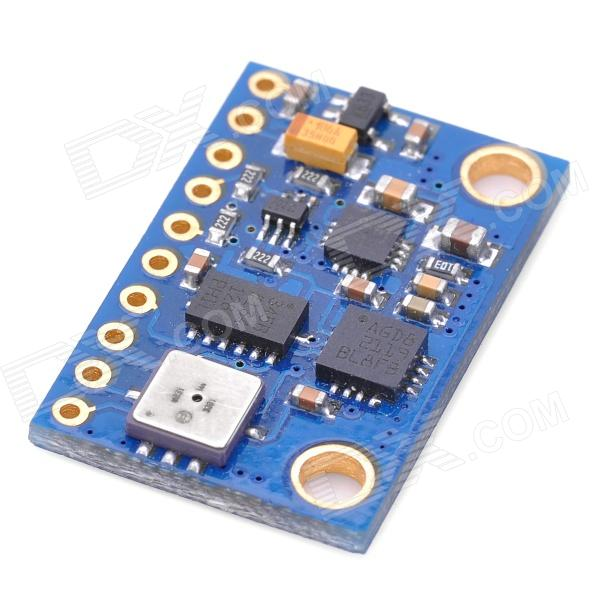
\includegraphics[width=0.18\columnwidth]{images/introduction/imu.jpg}
		}
		\subfloat[] 
		{
			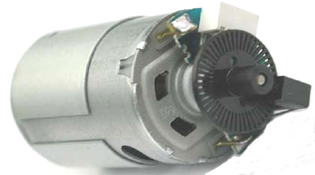
\includegraphics[width=0.2\columnwidth]{images/introduction/encoders-04.jpg}
		}\\
		\subfloat[]
		{
			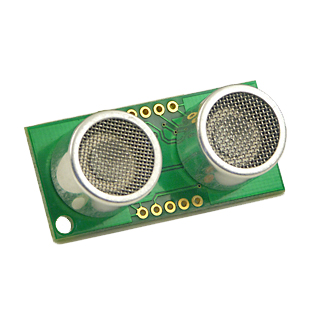
\includegraphics[width=0.22\columnwidth]{images/introduction/sonar.png}
		}
		\subfloat[]
		{
			\centering
			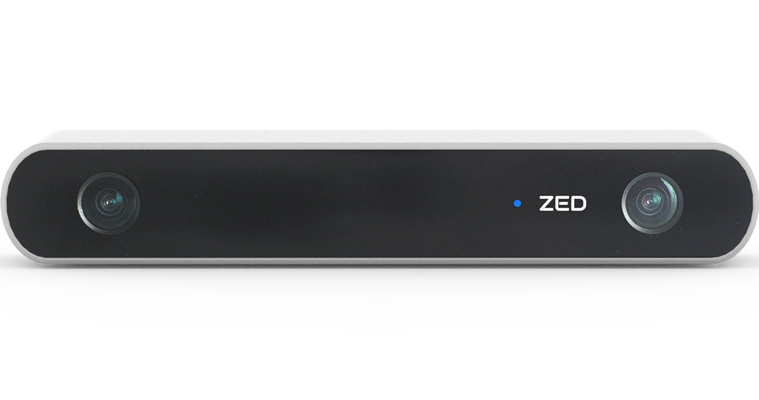
\includegraphics[width=0.3\columnwidth]{images/introduction/zed_camera2.png}
		}
		\subfloat[]
		{
			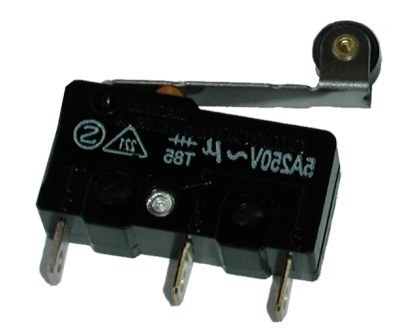
\includegraphics[width=0.16\columnwidth]{images/introduction/bumper.png}
		}
		\subfloat[]
		{
			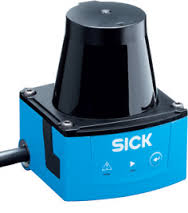
\includegraphics[width=0.16\columnwidth]{images/introduction/laser.jpg}
		}
	\end{figure}
\end{frame}


\subsection{SLAM Visual}


\begin{frame}
	\frametitle{SLAM Visual: Cámaras como sensores}
	
	¿Por qué utilizar cámaras?
       \begin{tabular}{cl}  
         \begin{tabular}{c}
           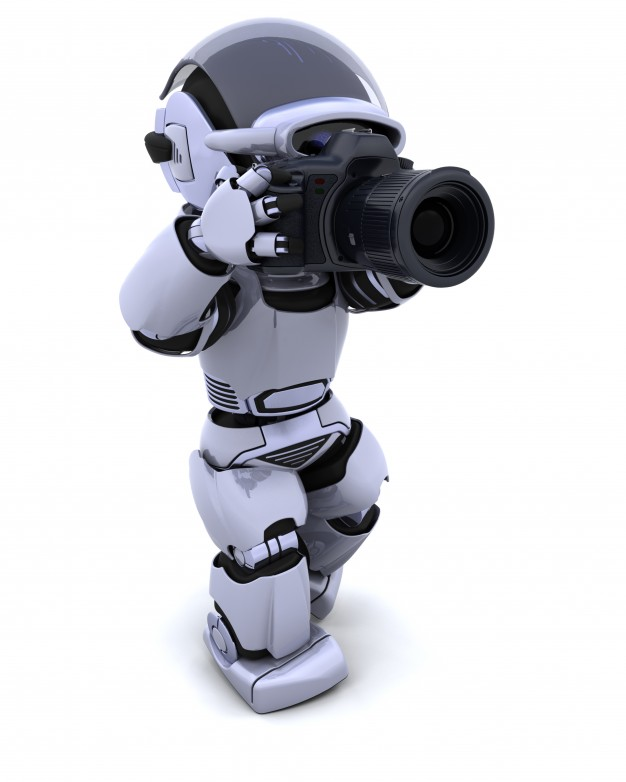
\includegraphics[width=0.3\columnwidth]{./images/robot-with-camera.jpg}
           \end{tabular}
           & \begin{tabular}{l}
             \parbox{0.5\linewidth}{
	            \begin{itemize}
	              	\pause
		            \item Rica información.
					\pause
		            \item Ambientes interiores y exteriores.
		            \pause
		            \item Sensores pasivos.
		            \pause
		            \item Bajo costo.
		            \pause
		            \item Portátiles.
		        \end{itemize}
		    }
        \end{tabular}  \\
	\end{tabular}
\end{frame}


\subsection{Cámaras}


\begin{frame}
	\frametitle{Reconstrucción 3D con una cámara}
	
	\pnote{
		Cámara = Mapeo punto 3D a píxel 2D\\
		Necesitamos 2 puntos de vista\\
		Necesitamos conocer el desplazamiento\\
	}
	% SPEECH:
	% hacer el ejemplo de cerrar un ojo y mover el dedo indice. Luego de mover el dedo caias veces notar que no conocemos su distancia.
	\only<1>{
		\begin{figure}[!h]
			\includegraphics[width=0.8\textwidth]{images/slam/monocularReconstruction1}
		\end{figure}
	}
	
	% SPEECH:
	% necesitamos dos puntos de vistas para poder realizar una reconstrucción 3D
	
	\only<2>{
		\begin{figure}[!h]
			\includegraphics[width=0.8\textwidth]{images/slam/monocularReconstruction2}
		\end{figure}
	}
	
	
	% SPEECH:
	% pero si estamos usando una sola camara y la movemos para tener dos puntos de vistas distintos, tenemos que saber cuanto se desplazo. Caso contrio, no vamos a poder saber si nos movimos poco, o si nos movimos mucho y las cosas estan muy lejos.
	
	\only<3>{
		\begin{figure}[!h]
			\includegraphics[width=0.8\textwidth]{images/slam/monocularReconstruction3}
		\end{figure}
	}
	
	\begin{block}{}
		Al utilizar una cámara, hay una ambig\"{u}edad sobre la escena que se esta observando.
	\end{block}
	
\end{frame}


\begin{frame}
	\frametitle{¿Y si tenemos dos cámaras?}
	
	\pnote{
		Permiten recuperar la profundidad de la escena con una única captura.\\
		Permiten conocer la escala real de la escena observada.\\
	}
	
	\begin{figure}[!h]
		\includegraphics[width=0.6\textwidth]{images/slam/stereoReconstruction}
	\end{figure}
	
	\begin{block}{}
		Si tenemos {\bf dos cámaras}, y se conoce la posición de una con respecto a la otra, es posible realizar una reconstrucción 3D sin ambig\"{u}edades.
	\end{block}
	
\end{frame}


% Frame ---------------------------------------------------------------------
\begin{frame}
    \frametitle{Geometría estéreo: Disparidad}
    \pnote{
	    Distancia existente entre las proyecciones de las diferentes cámaras.\\
	    La profundidad z es inversamente proporcional a la disparidad d.\\
    }
    
    \begin{figure}[!htb]
        \centering
        \subfloat[]{
        \hspace{-3.0em}
        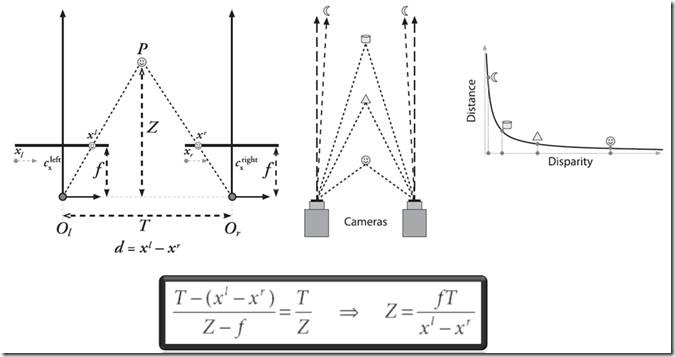
\includegraphics[width=1.15\columnwidth]{./images/disparity_sketch.jpeg}}
        \hfill
        \centering

        \hfill
    \end{figure}

\end{frame}


% Frame ---------------------------------------------------------------------
\begin{frame}
    \frametitle{Cierre y Motivación}
    \pnote{
    	Robótica móvil.\\
		Navegación autónoma.\\
		SLAM.\\
		SLAM Visual.\\
		Trayectoria seguro: mapa denso!\\
    }
    
    \begin{block}{}
    \centering
	Mapeo denso online sobre sistemas SLAM basados en visión estéreo
	\end{block}

	\begin{figure}[!htb]
		\captionsetup{justification=centering}
		\subfloat[S-PTAM]{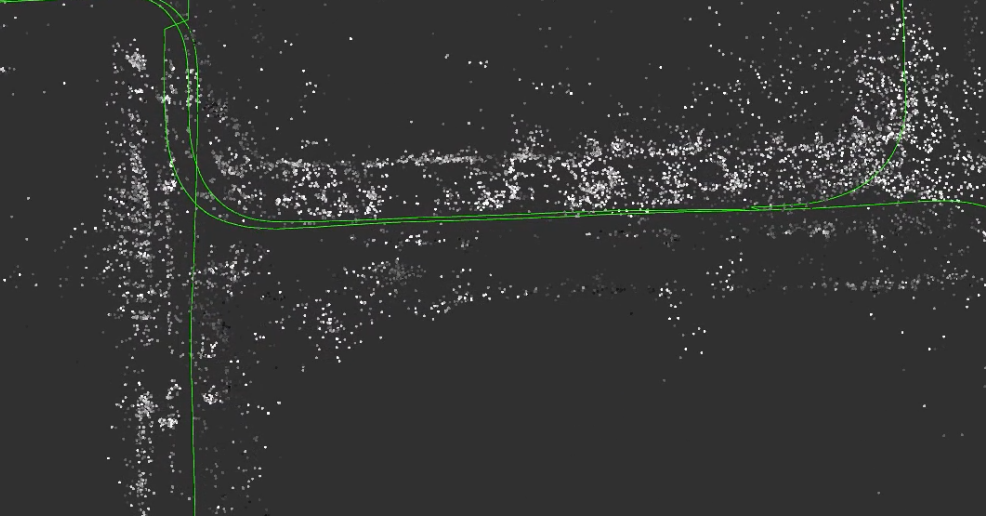
\includegraphics[width=0.4\columnwidth,height=2.5cm]{./introduction/sptam-map.png}
		}
		\hfil
		\subfloat[S-PTAM Denso]{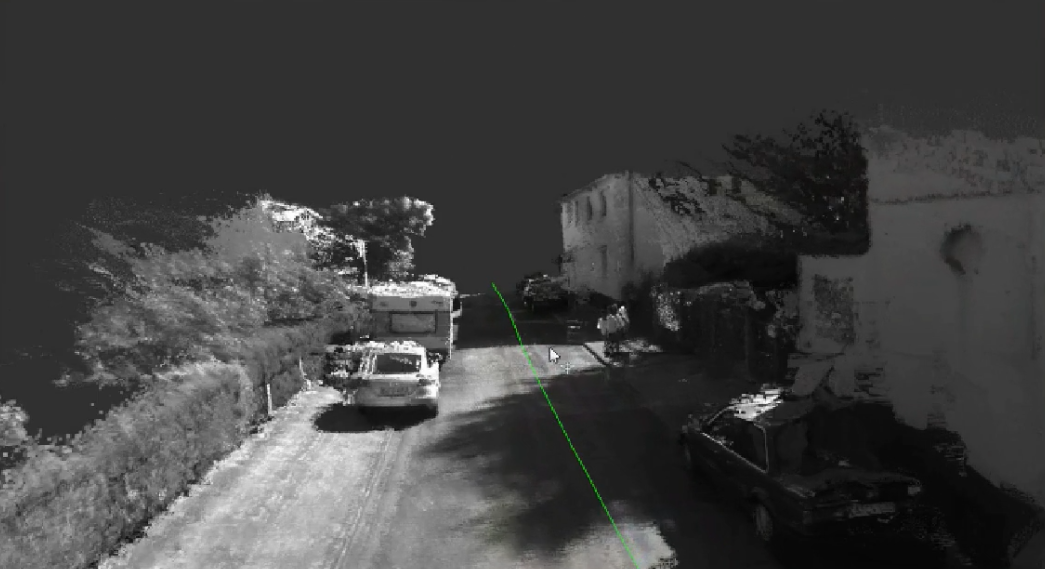
\includegraphics[width=0.4\columnwidth,height=2.5cm]{./introduction/dense-map.png}
		}
	\end{figure}
	
\end{frame}


\section{S-PTAM Denso}


\subsection{S-PTAM}


\fullFrameMovie[loop]{~/Videos/S-PTAM.mkv}{./images/S-PTAM-video-cover.png}{
	\frametitle{S-PTAM: Stereo Parallel Tracking and Mapping}
	\pnote{
    	Sensor: Cámara estéreo\\
		Construye y mantiene un mapa disperso del entorno.\\
        Sistema SLAM basado en features.\\
		Basado en keyframes.\\
        Fuertemente paralelizado: tracking, local mapping y loop closing.\\
        Real-time incluso en trayectorias largas.\\
        Código open-source en ROS (GPLv3) https://github.com/lrse/sptam\\
	}

}


\subsection{Funcionamiento}


% Frame ---------------------------------------------------------------------
\begin{frame}
	\frametitle{S-PTAM Denso}
	\pnote{
		Aporte de la tesina.\\
		Breve resumen.\\
	}	
	
	\begin{figure}[htb]
		\centering
		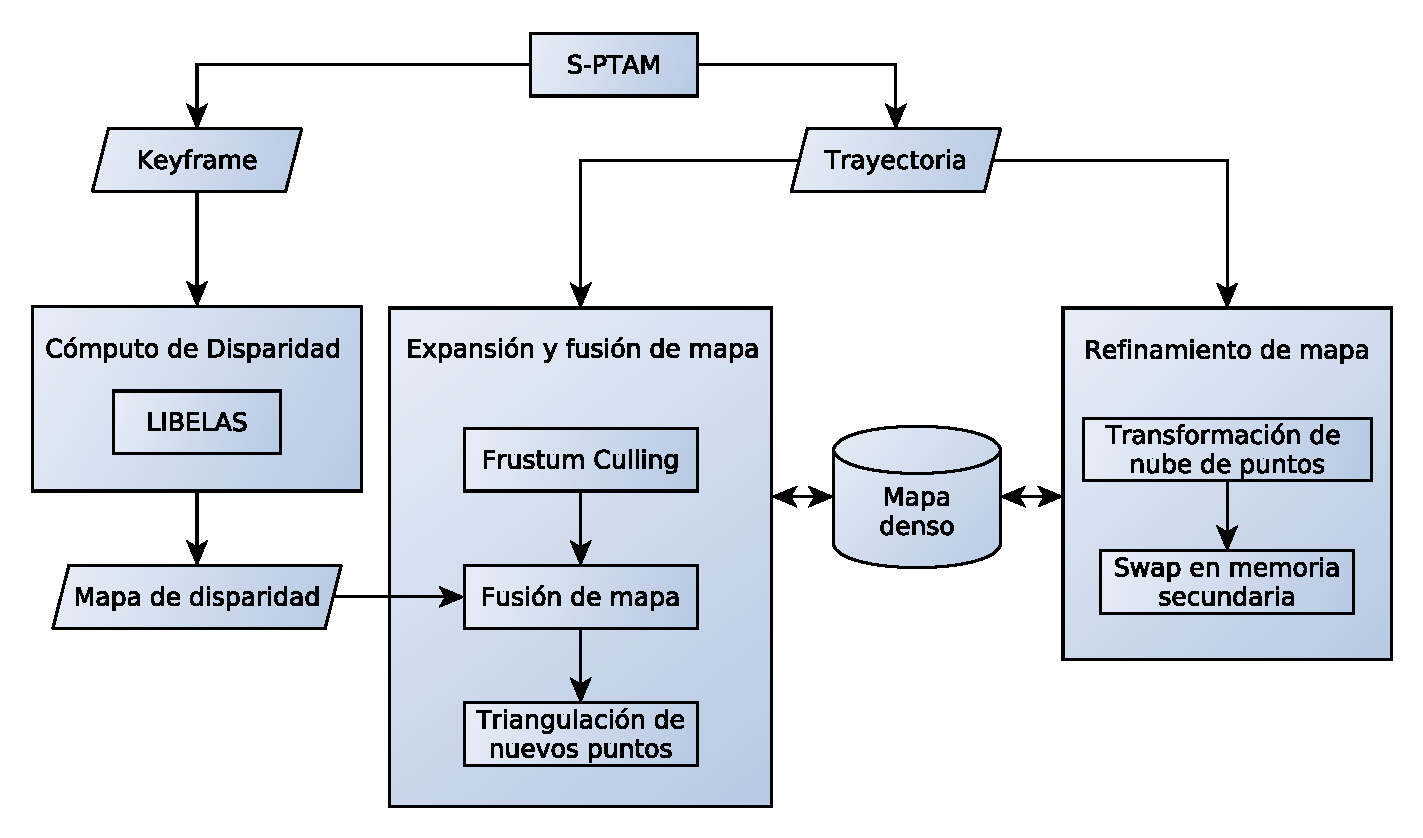
\includegraphics[width=1.0\columnwidth]{./method/metodo-diagram.pdf}
		\hfill
	\end{figure}
\end{frame}


% Frame ---------------------------------------------------------------------
\begin{frame}
	\frametitle{Mapa de disparidad}
	\pnote{
		LIBELAS: librería mapa denso.\\
		Usa todos los píxeles, contiene error (cielo).\\
	}	

	\begin{itemize}
		\item Computa mapa de disparidad del \emph{keyframe} actual $\keyframe_{j}$.
	\end{itemize}
	
	\begin{figure}[htb]
		\centering
		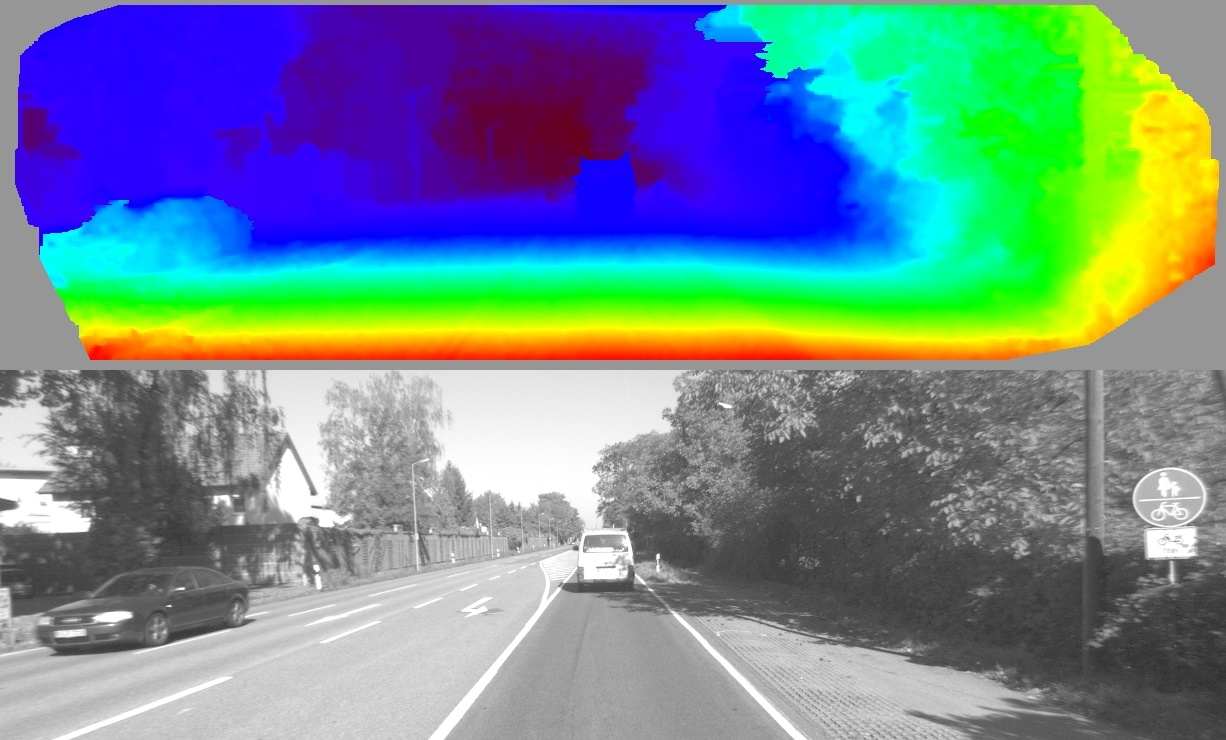
\includegraphics[width=0.4\columnwidth]{method/libelas_merge_kitti04_22.jpg}
		\caption{Mapa de disparidad LIBELAS - Dataset KITTI}
	\end{figure}

	\vspace{-1em}

	\begin{figure}[htb]
		\centering
		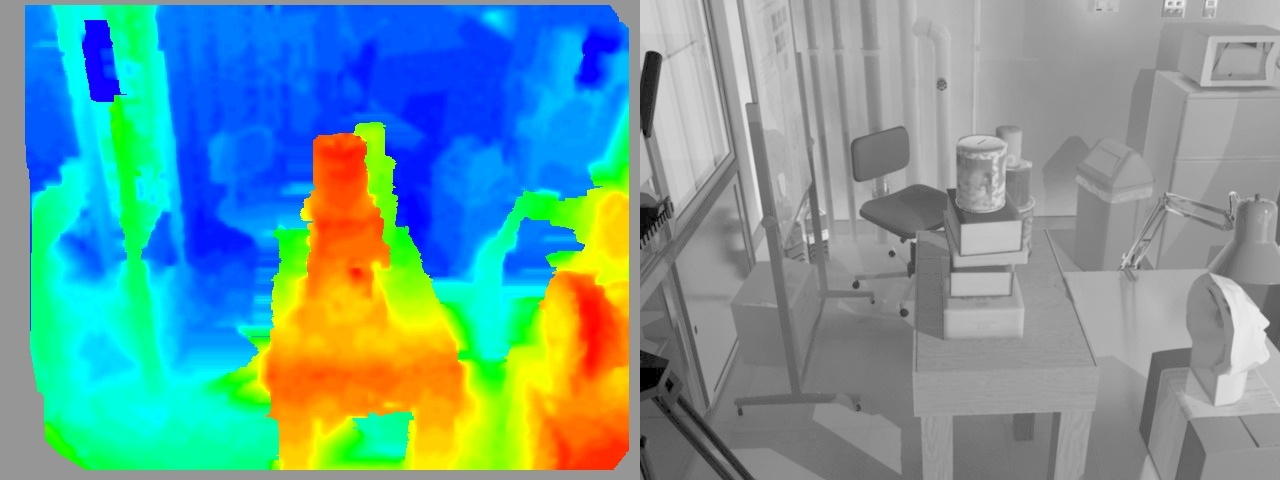
\includegraphics[width=0.4\columnwidth]{method/libelas_merge_tsukuba_222.jpg}
		\caption{Mapa de disparidad LIBELAS - Dataset Tsukuba}
	\end{figure}

	\begin{itemize}
		\item Colores: (rojo: mayor disparidad, azul: menor disparidad).
	\end{itemize}
	
\end{frame}


% Frame ---------------------------------------------------------------------
\begin{frame}
	\frametitle{Expansión y fusión de mapa: Heurística de fusión}
	\begin{figure}[htb]
		\centering
		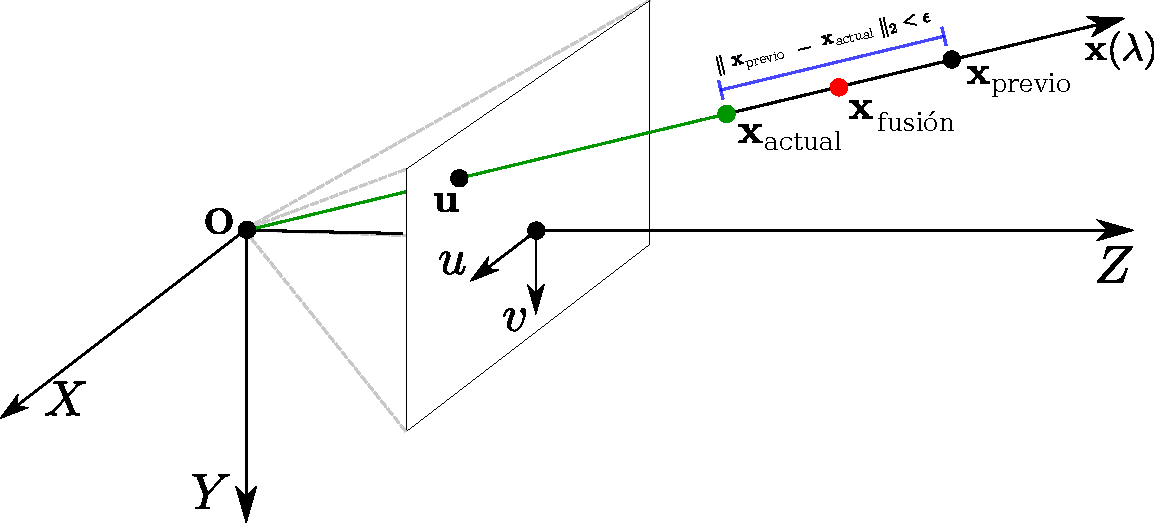
\includegraphics[width=\columnwidth]{method/metodo-fusion-spa.pdf}
	\end{figure}
	\begin{equation*}
		\point_{fusi\acute{o}n}=\frac{1}{\inverseDepth_{fusi\acute{o}n}}\frac{\point_{actual}}{\norm{\point_{actual}}}
		\quad \text{donde} \quad 
		\inverseDepth_{fusi\acute{o}n}=\frac{\inverseDepth_{actual}+\inverseDepth_{previo}}{2}
	\end{equation*}
\end{frame}


%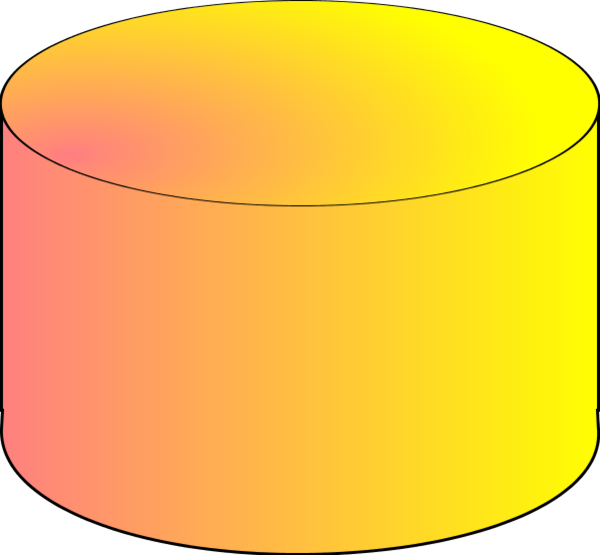
\includegraphics[width=0.2\columnwidth]{./images/swap-memory.png}

\begin{frame}
	\frametitle{Refinamiento de mapa}
	
	\pnote{
		Transforma nubes de puntos cuando la posición del keyframe asociado es actualizada.\\
		Comportamiento esperable en sistemas de SLAM, que refinan la trayectoria a lo largo de la secuencia.\\
		Nubes de puntos en RAM hasta que salen del mapa local.\\
		Permite correr en secuencias de extensa longitud.\\
	}    
	
       \begin{tabular}{cl}  
           \begin{tabular}{c}
           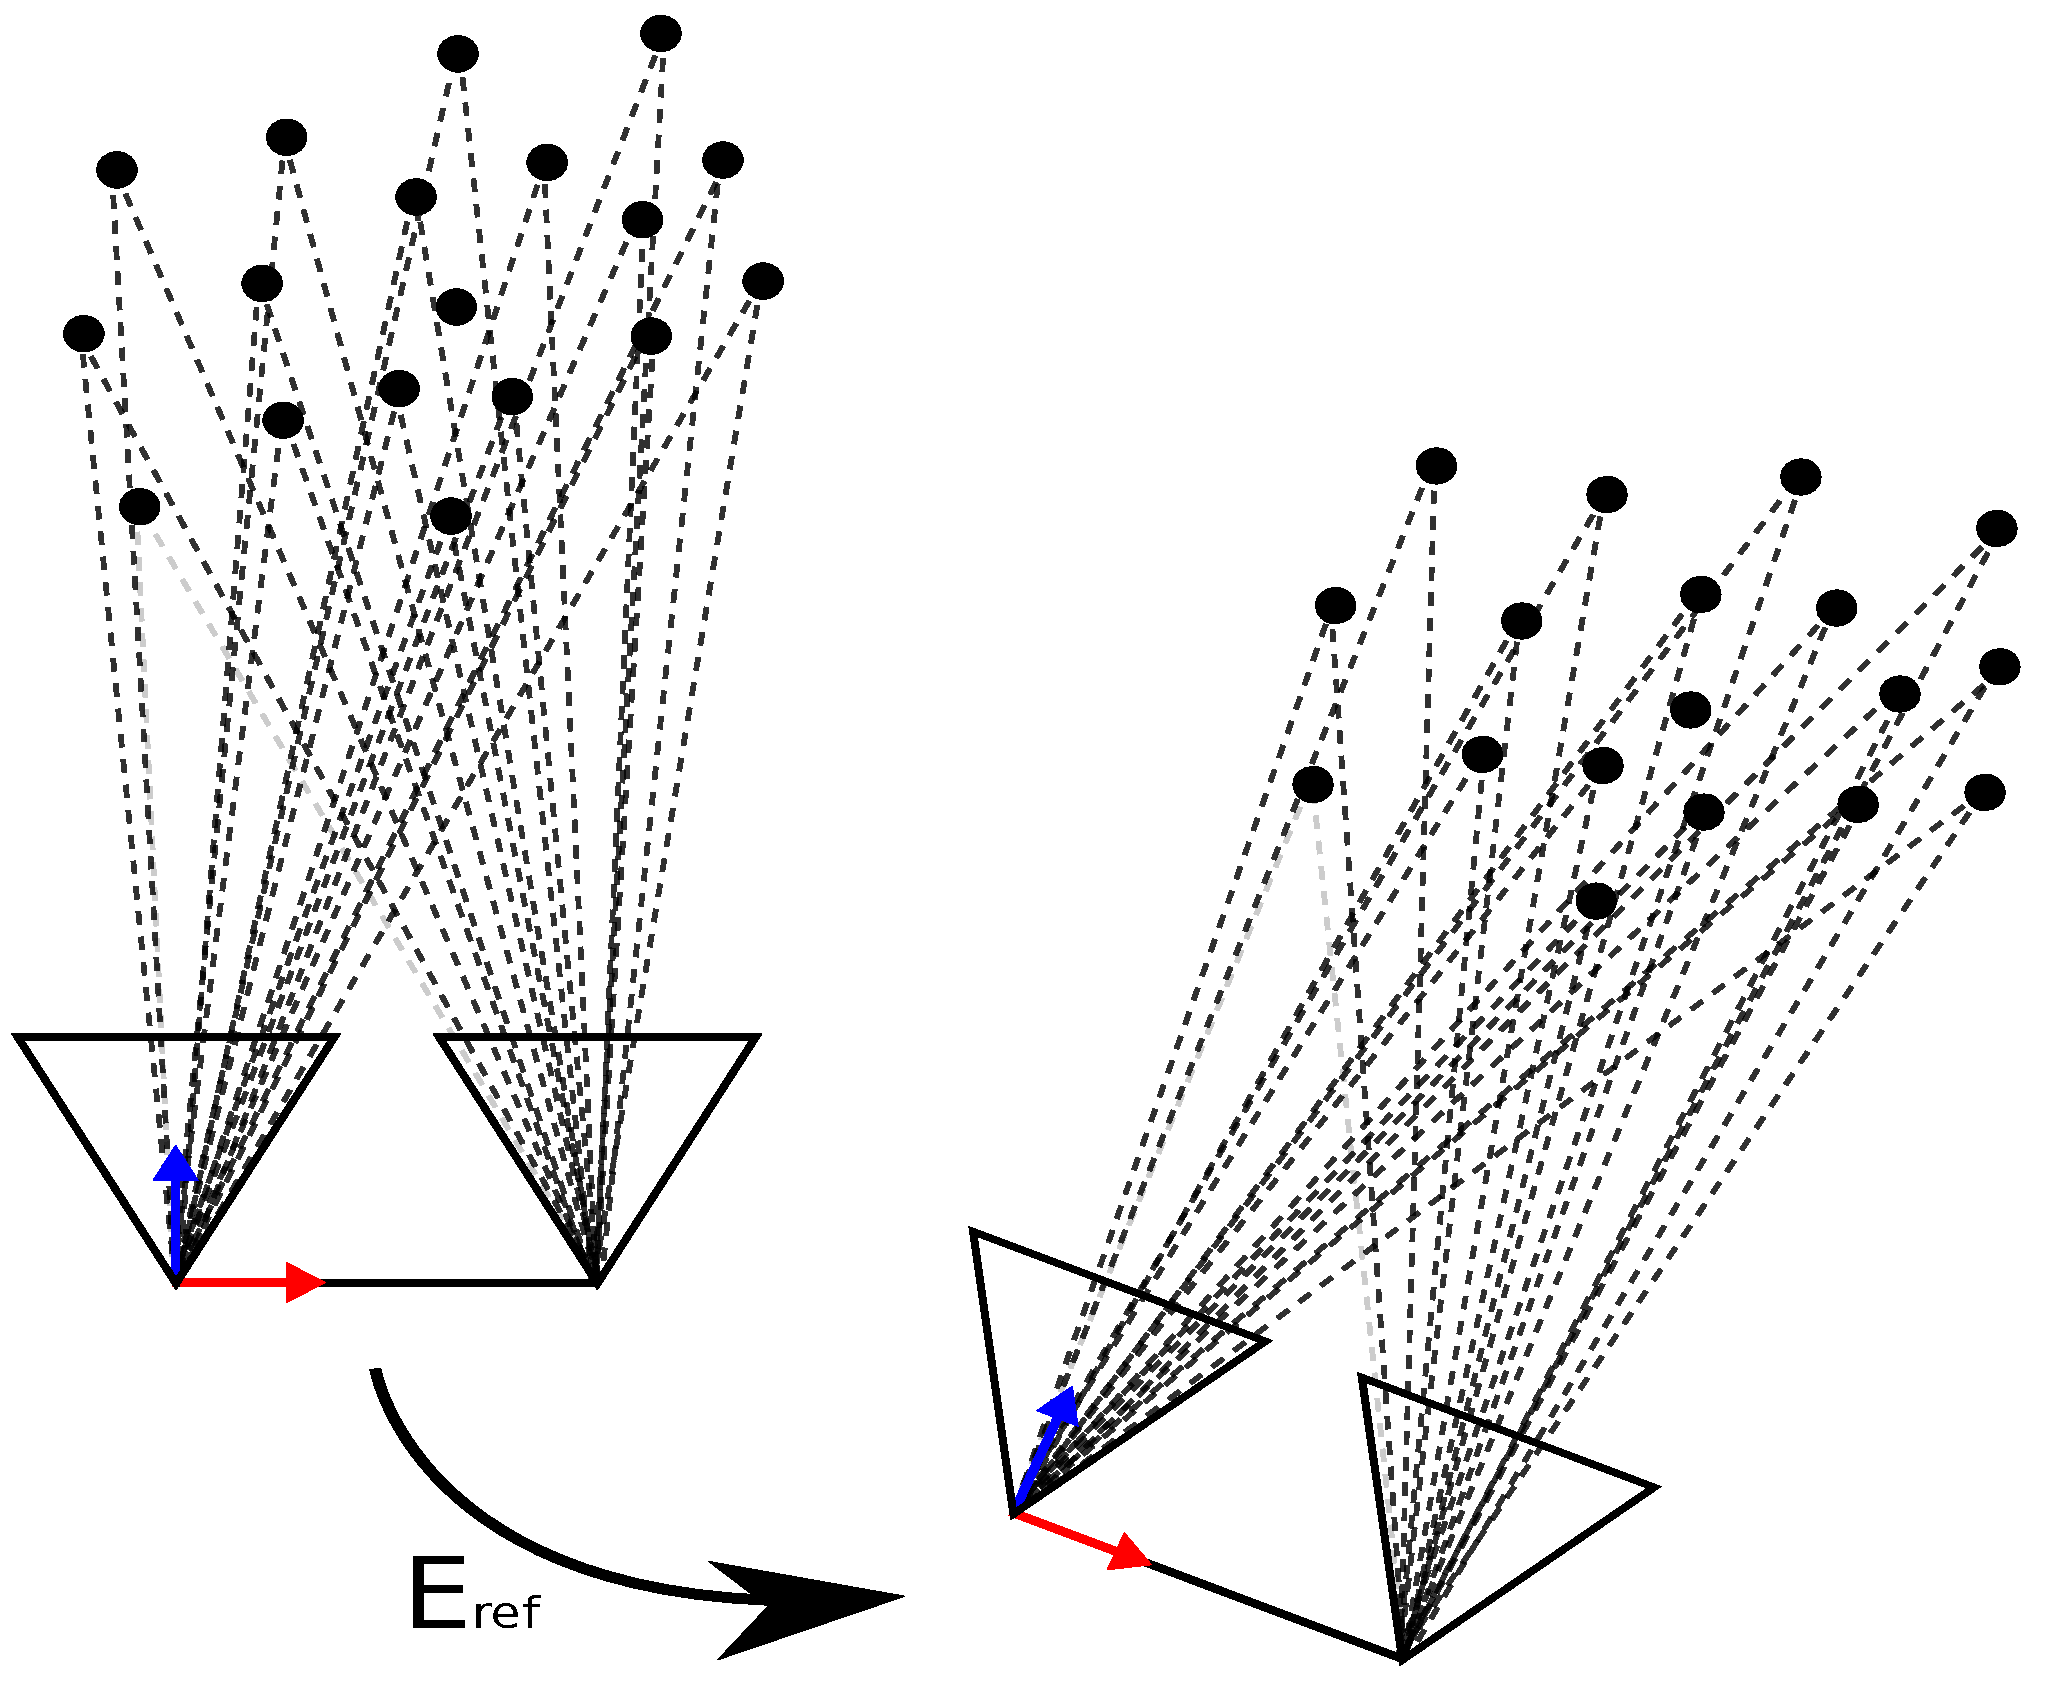
\includegraphics[width=0.5\columnwidth]{./images/point_cloud_refinement.pdf}
           \end{tabular}
           & \begin{tabular}{l}
             \parbox{0.5\linewidth}{
	            \begin{itemize}
	            	\item Refinamiento de nubes de puntos.
	            	\item Swapping del mapa en memoria secundaria.
		        \end{itemize}
		    }
			\end{tabular}
		\end{tabular}
		
		\begin{figure}[!htb]
		\captionsetup{justification=centering}
		\subfloat[SWAP memory]{
			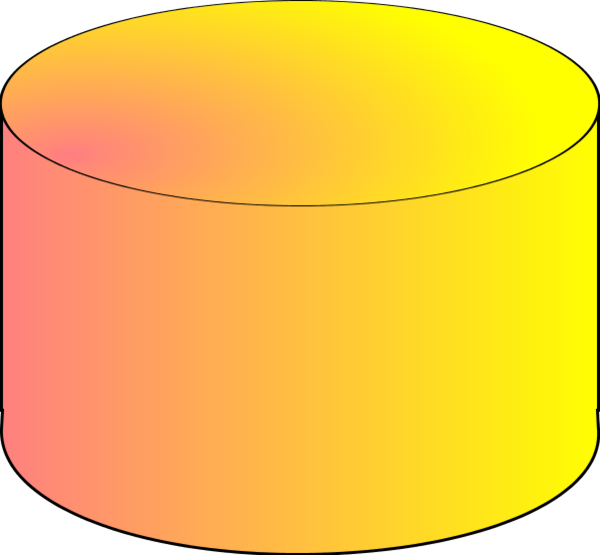
\includegraphics[width=0.15\columnwidth]{./images/swap-memory.png}
		}
		\end{figure}
\end{frame}


\subsection{Implementación}


% Frame ---------------------------------------------------------------------
\begin{frame}
	\frametitle{Framework}
	

	\begin{figure}[htb]
		\subfloat[] {
			\begin{tabular}[b]{c}
				\centering
				$\vcenter{\hbox{
\includegraphics[width=0.15\columnwidth]{./method/opencv.png}}}$
				\hspace{1em}
				$\vcenter{\hbox{
\includegraphics[width=0.40\columnwidth]{./method/ros.png}}}$
				\hspace{1em}
				$\vcenter{\hbox{
\includegraphics[width=0.28\columnwidth]{./method/pcl.png}}}$
			\end{tabular}
		}
	\end{figure}
	
	\vfill
	\begin{tiny}
		Código fuente disponible públicamente bajo licencia (GPLv3) \url{https://github.com/CIFASIS/dense-sptam}.
	\end{tiny}
	
	\pnote{
		Conjunto de frameworks para desarrollo de software en robótica.\\
		Abstracción del hardware.\\
	    Control de dispositivos de bajo nivel.\\
	    Arquitectura: Cada nodo es una unidad de ejecución. Comunicación entre nodos mediante mensajes.
		Mantenimiento de paquetes.\\
	    Utilizado en la comunidad robótica.\\
		Implementado como un nodo ROS.\\
		OpenCV: manejo y codificación de imágenes.\\
		Point Cloud Library (PCL): manejo de nubes de puntos.\\
		LIBELAS: cómputo de mapas de disparidad.\\
		Compuesto de 3 hilos de ejecución paralela.\\
	}

\end{frame}


\section{Evaluación}


\subsection{Datasets}


% Frame ---------------------------------------------------------------------
\begin{frame}
	\frametitle{Dataset KITTI}

	\begin{figure}
		\subfloat[] {
			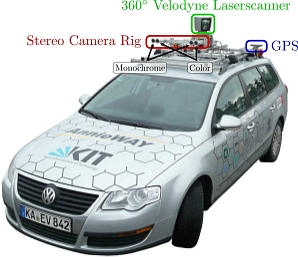
\includegraphics[width=0.3\columnwidth]{./images/kitti_sensors}
		}\hfill{}
		\subfloat[] {
			\begin{tabular}[b]{c}%
				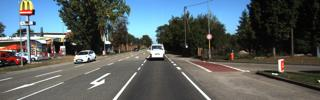
\includegraphics[width=0.3\columnwidth]{./images/kitti01}\thickspace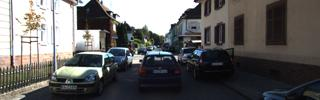
\includegraphics[width=0.3\columnwidth]{./images/kitti02}\\
				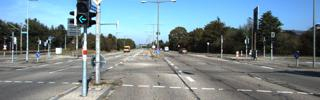
\includegraphics[width=0.3\columnwidth]{./images/kitti03}\thickspace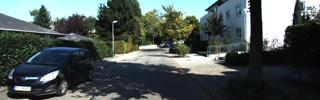
\includegraphics[width=0.3\columnwidth]{./images/kitti04}\\
				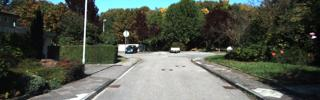
\includegraphics[width=0.3\columnwidth]{./images/kitti05}\thickspace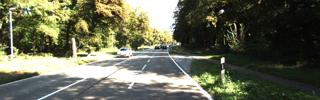
\includegraphics[width=0.3\columnwidth]{./images/kitti06}
			\end{tabular}
		}
	\end{figure}

	\begin{itemize}
        \item Ambientes exteriores (trayectorias de varios kilómetros)
        \item 1344$\times$391@10Hz, baseline: 60cm
    \end{itemize}

\end{frame}


% Frame ---------------------------------------------------------------------
\begin{frame}
	\frametitle{Dataset Tsukuba}

	\begin{figure}
		\subfloat[] {
			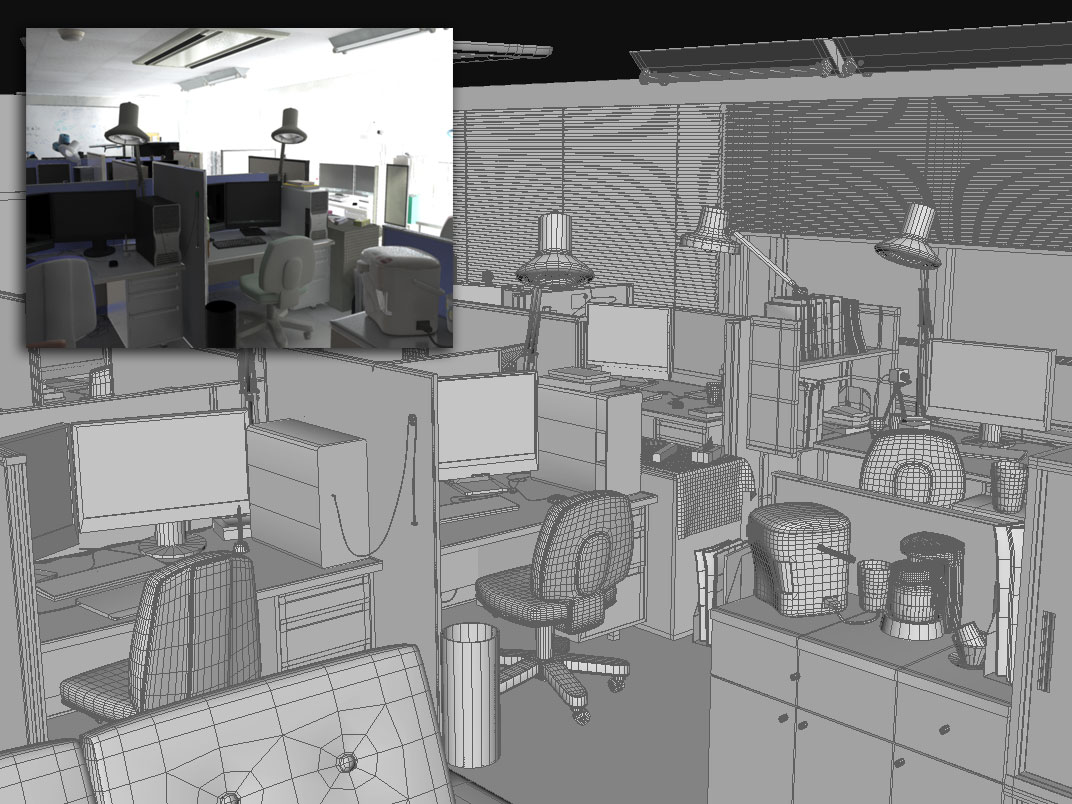
\includegraphics[width=0.41\columnwidth]{./images/tsukuba_dataset}
		}\hspace{0.2cm}
		\subfloat[] {
			\begin{tabular}[b]{c}%
				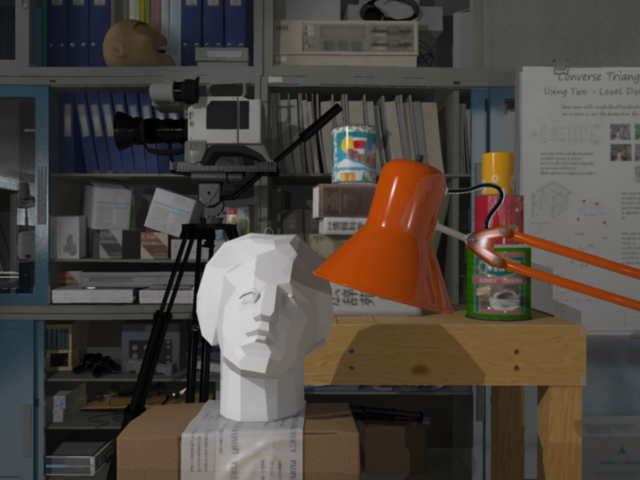
\includegraphics[width=0.2\columnwidth]{./images/tsukuba_sample1}\thickspace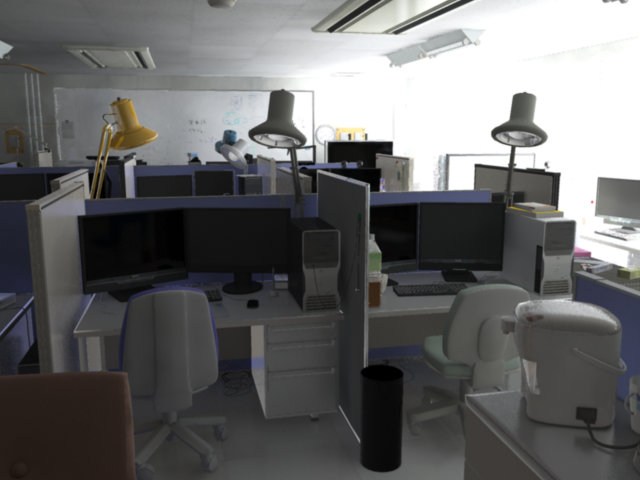
\includegraphics[width=0.2\columnwidth]{./images/tsukuba_sample2}\\
				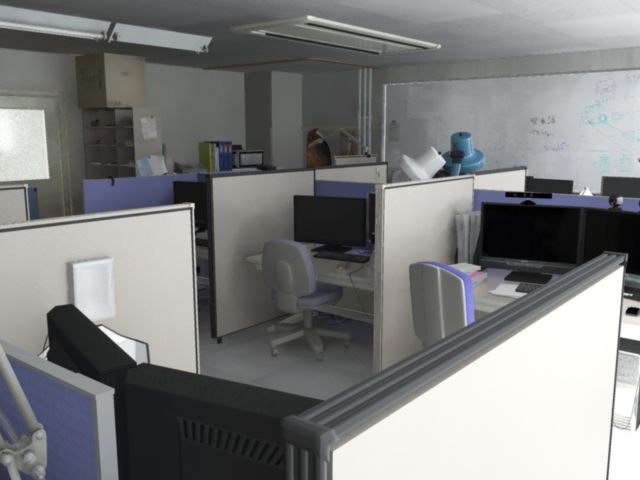
\includegraphics[width=0.2\columnwidth]{./images/tsukuba_sample3}\thickspace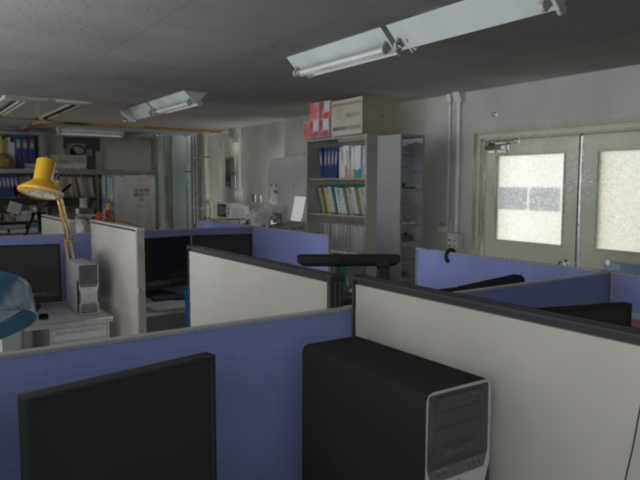
\includegraphics[width=0.2\columnwidth]{./images/tsukuba_sample4}
			\end{tabular}
		}
	\end{figure}
	
	\begin{itemize}
        \item Ambiente interior (sintético)
        \item 640$\times$480@30Hz, baseline: 10cm
    \end{itemize}
    
\end{frame}


% Frame ---------------------------------------------------------------------
\begin{frame}
	\frametitle{Reconstrucción 3D: Tsukuba}
	\begin{figure}
		\subfloat[] {
			\begin{tabular}[b]{c}
				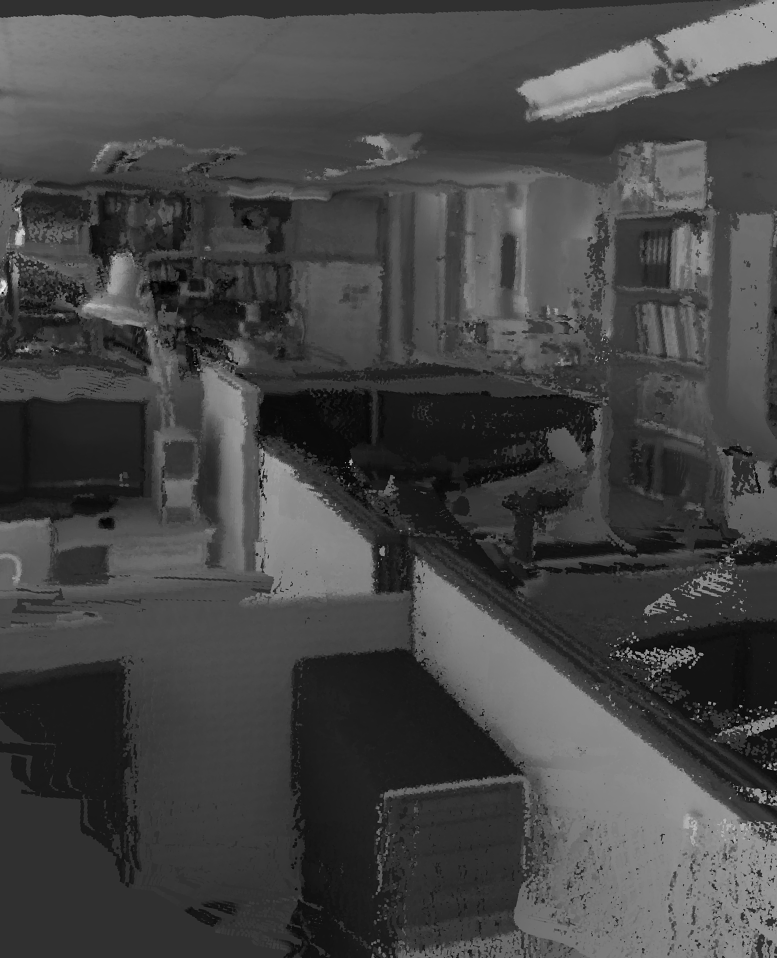
\includegraphics[width=0.3\columnwidth,height=3.0cm]{./images/tsukuba_3d_1}\thickspace
				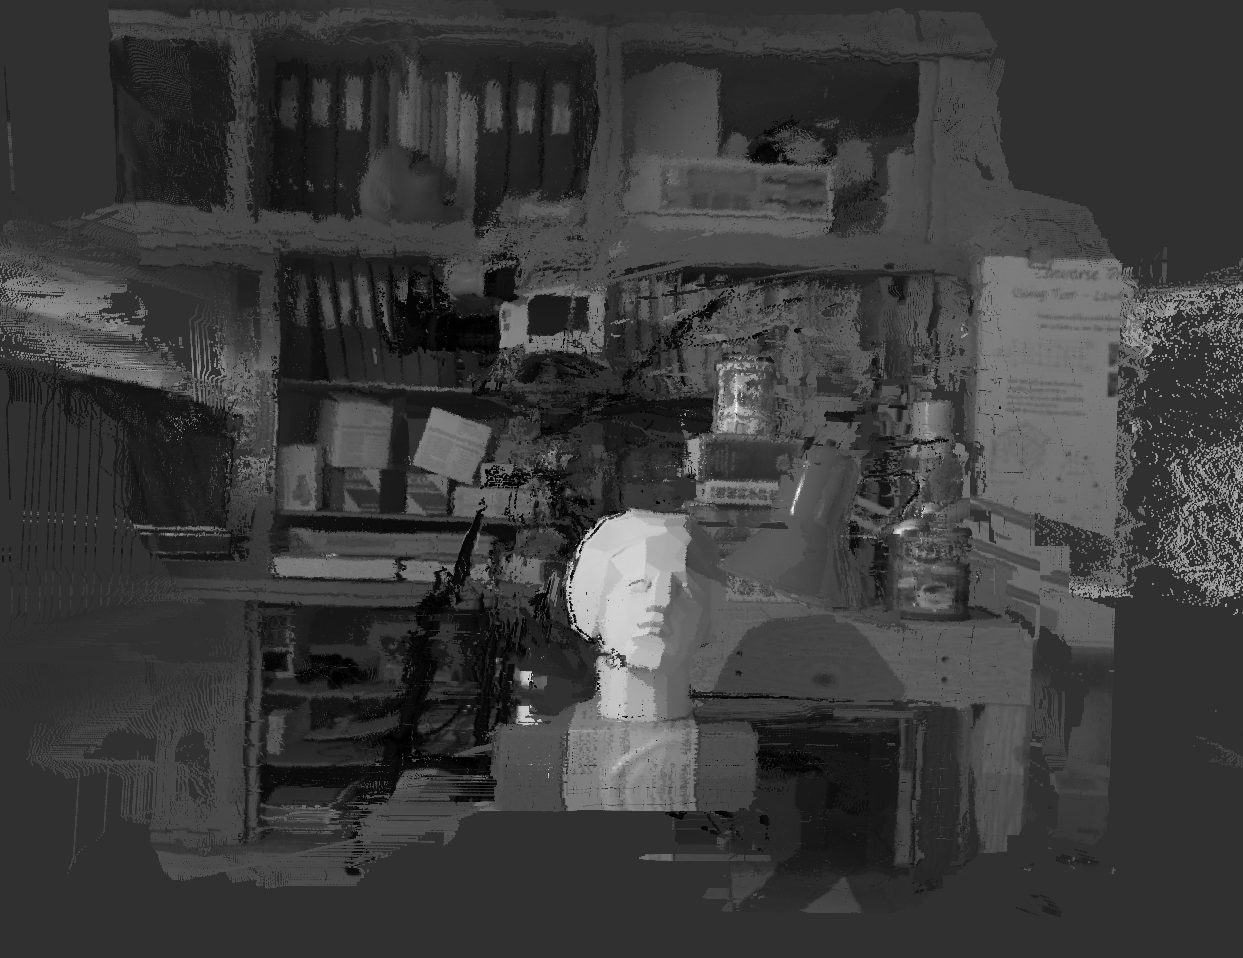
\includegraphics[width=0.3\columnwidth,height=3.0cm]{./images/tsukuba_3d_2}\thickspace
				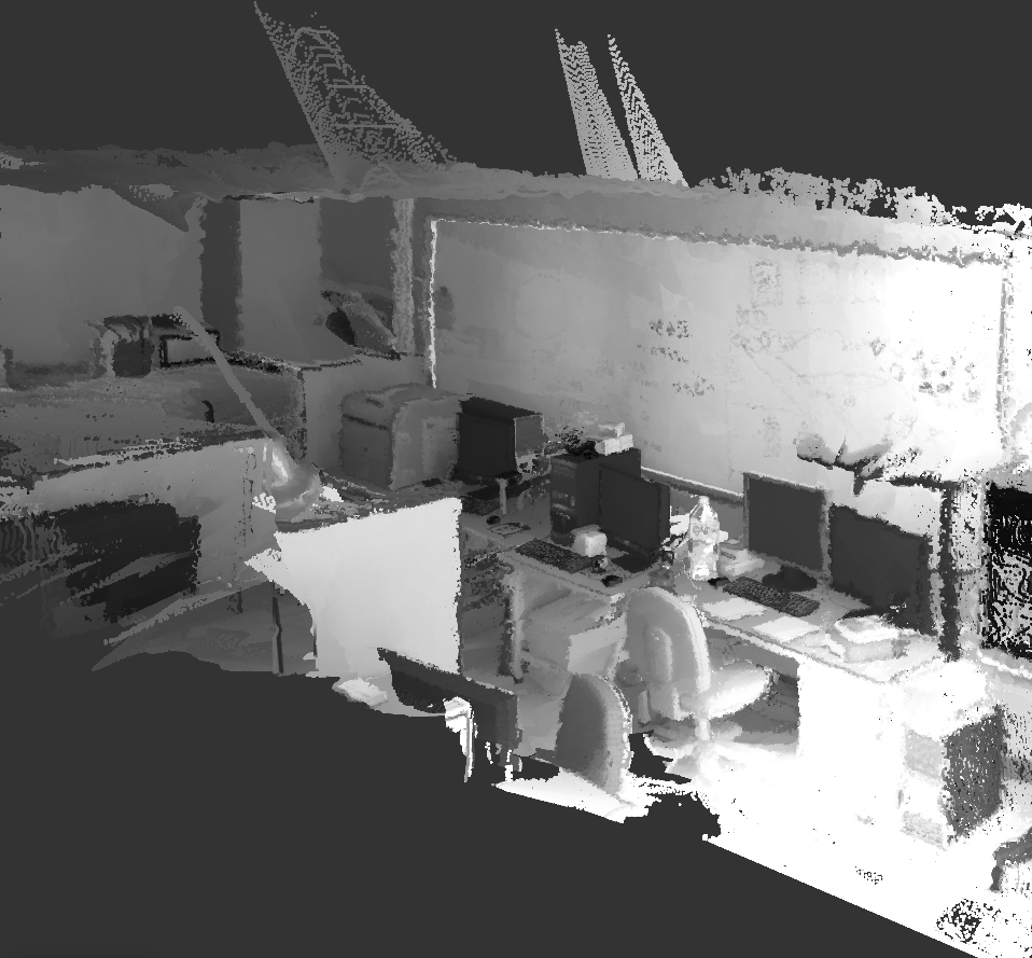
\includegraphics[width=0.3\columnwidth,height=3.0cm]{./images/tsukuba_3d_3}
			\end{tabular}
		}
	\end{figure}
\end{frame}


% Frame ---------------------------------------------------------------------
\begin{frame}
	\frametitle{Reconstrucción 3D: KITTI}
    Video S-PTAM Denso: KITTI Sequence 06
\end{frame}


\subsection{Resultados}


% Frame ---------------------------------------------------------------------
\begin{frame}
	\frametitle{KITTI: error de reconstrucción}
	\pnote{
		Comparación de mapas de profundidad.\\
		Proyectamos nubes de puntos.\\
		LIBELAS.\\
		GT en KITTI y Tsukuba.\\
	}	
	
	\vspace{-2em}
	\begin{figure}
		\subfloat[Imagen izquierda]{
			\begin{tabular}[b]{c}
				\includegraphics[width=0.45\columnwidth]{./experiments/kitti06_frame612_rgb.png}
			\end{tabular}
		}\thickspace
		\subfloat[Ground-Truth]{
			\begin{tabular}[b]{c}
				\includegraphics[width=0.45\columnwidth]{./experiments/kitti06_frame612_gt_high50.png}
			\end{tabular}
		}
	\end{figure}
	\vspace{-2em}
	\begin{figure}
		\subfloat[Mapa profundidad LIBELAS]{
			\begin{tabular}[b]{c}
				\includegraphics[width=0.45\columnwidth]{./experiments/kitti06_frame612_libelas_depth_high50-m.png}
			\end{tabular}
		}\thickspace
		\subfloat[Error mapa profundidad LIBELAS]{
			\begin{tabular}[b]{c}
				\includegraphics[width=0.45\columnwidth]{./experiments/kitti06_frame612_libelas_error_high50-m.png}
			\end{tabular}
		}
	\end{figure}
	\vspace{-2em}
	\begin{figure}
		\subfloat[Mapa profundidad S-PTAM Denso]{
			\begin{tabular}[b]{c}
				\includegraphics[width=0.45\columnwidth]{./experiments/kitti06_frame612_dense_high50-m.png}
			\end{tabular}
		}\thickspace
		\subfloat[Error mapa profundidad S-PTAM Denso]{
			\begin{tabular}[b]{c}
				\includegraphics[width=0.45\columnwidth]{./experiments/kitti06_frame612_error_high50-m.png}
			\end{tabular}
		}
	\end{figure}
	\vspace{-2em}
	\begin{figure}
		\subfloat[]{
			\begin{tabular}[b]{c}
				\includegraphics[width=0.60\columnwidth]{./experiments/high50_bar.pdf}
			\end{tabular}
		}
	\end{figure}
\end{frame}


% Frame ---------------------------------------------------------------------
\begin{frame}
	\frametitle{Tsukuba: error de reconstrucción}
	\vspace{-1em}
	\begin{figure}
		\captionsetup{justification=centering}
		\subfloat[Imagen izquierda]{
			\begin{tabular}[b]{c}
				\includegraphics[width=0.25\columnwidth]{./experiments/tsukuba_frame807_rgb.png}
			\end{tabular}
		}\thickspace
		\subfloat[Mapa profundidad LIBELAS]{
			\begin{tabular}[b]{c}
				\includegraphics[width=0.25\columnwidth]{./experiments/tsukuba_frame807_libelas_depth_high6.png}
			\end{tabular}
		}\thickspace
		\subfloat[Mapa profundidad S-PTAM Denso]{
			\begin{tabular}[b]{c}
				\includegraphics[width=0.25\columnwidth]{./experiments/tsukuba_frame807_dense_high6.png}
			\end{tabular}
		}
	\end{figure}
	\vspace{-2em}
	\begin{figure}
		\captionsetup{justification=centering}
		\subfloat[Ground-Truth]{
			\begin{tabular}[b]{c}
				\includegraphics[width=0.25\columnwidth]{experiments/tsukuba_frame807_gt_high6.png}
			\end{tabular}
		}\thickspace
		\subfloat[Error mapa profundidad LIBELAS]{
			\begin{tabular}[b]{c}
				\includegraphics[width=0.25\columnwidth]{./experiments/tsukuba_frame807_libelas_error_high6-m.png}
			\end{tabular}
		}\thickspace
		\subfloat[Error mapa profundidad S-PTAM Denso]{
			\begin{tabular}[b]{c}
				\includegraphics[width=0.25\columnwidth]{./experiments/tsukuba_frame807_error_high6-m.png}
			\end{tabular}
		}
	\end{figure}
	\vspace{-2em}
	\begin{figure}
		\subfloat[]{
			\begin{tabular}[b]{c}
				\includegraphics[width=0.60\columnwidth]{./experiments/high6_bar.pdf}
			\end{tabular}
		}
	\end{figure}
\end{frame}


% Frame ---------------------------------------------------------------------
\begin{frame}
	\frametitle{KITTI 06: error de mediana}
	\centering
	Error (profundidad vs. error) en la secuencia 06 del Dataset KITTI.
	\begin{figure}[!htb]
		\captionsetup{justification=centering}
		\subfloat[Error en LIBELAS]{\includegraphics[width=0.48\columnwidth]{./experiments/kitti06_libelas_boxplot.png}%
		}
		\hfil
		\subfloat[Error en S-PTAM Denso]{\includegraphics[width=0.48\columnwidth]{./experiments/kitti06_dense_boxplot.png}%
		}
	\end{figure}
\end{frame}


% Frame ---------------------------------------------------------------------
\begin{frame}
	\frametitle{KITTI 06: error de mediana}
	\vspace{-2em}
	\begin{figure}[!htb]
		\captionsetup{justification=centering}
		\subfloat[Comparación de mediana de error entre LIBELAS y S-PTAM Denso (profundidad vs. error) en la secuencia 06 del Dataset KITTI.] {
			\includegraphics[width=0.8\columnwidth]{./experiments/medians_comparison_kitti.png}%
		}
	\end{figure}
\end{frame}


% Frame ---------------------------------------------------------------------
\begin{frame}
	\frametitle{Tsukuba: error de mediana}
	\centering
	Error (profundidad vs. error) en el Dataset Tsukuba.
	\begin{figure}[!htb]
		\captionsetup{justification=centering}
		\subfloat[Error en LIBELAS]{\includegraphics[width=0.48\columnwidth]{./experiments/tsukuba_libelas_boxplot.png}%
		}
		\hfil
		\subfloat[Error en S-PTAM Denso]{\includegraphics[width=0.48\columnwidth]{./experiments/tsukuba_dense_boxplot.png}%
		}
	\end{figure}
\end{frame}


% Frame ---------------------------------------------------------------------
\begin{frame}
	\frametitle{Tsukuba: error de mediana}
	\vspace{-2em}
	\begin{figure}[!htb]
		\captionsetup{justification=centering}
		\subfloat[Comparación de mediana de error entre LIBELAS y S-PTAM Denso (profundidad vs. error) en el Dataset Tsukuba.] {
			\includegraphics[width=0.8\columnwidth]{./experiments/medians_comparison_tsukuba.png}%
		}
	\end{figure}
\end{frame}


% Frame ---------------------------------------------------------------------
\begin{frame}
	\frametitle{Cantidad de puntos}
	\begin{figure}[!htb]
		\centering
		\subfloat[KITTI]{\includegraphics[width=0.5\columnwidth]{./experiments/points_kitti06}%
			}
		\hfil
		\subfloat[Tsukuba]{\includegraphics[width=0.5\columnwidth]{./experiments/points_tsukuba}%
			}
	\end{figure}
\end{frame}


% Frame ---------------------------------------------------------------------
\begin{frame}
	\frametitle{S-PTAM Denso!}
	Video S-PTAM Denso: KITTI Sequences (varias).
\end{frame}


\section{Conclusiones y trabajos futuros}


% Frame ---------------------------------------------------------------------
\begin{frame}
	\frametitle{Conclusiones}
	\begin{itemize}
		\item Sistema de SLAM capaz de generar un \textbf{mapa local denso} de manera \textbf{online}.
        \item La \textbf{precisión} es útil para tareas de navegación.
        \item Funciona incluso en trayectorias de \textbf{grandes dimensiones}.
        \item Evaluado en \textbf{datasets} públicos: KITTI (outdoors) y Tsukuba (indoors).
	    \item Código open-source en ROS (GPLv3) \url{https://github.com/CIFASIS/dense-sptam}
	    \item Nodo ROS \textbf{reutilizable}, desacoplado del sistema de SLAM disperso.
	  	\item Explota \textbf{paralelismo}.
	  	\item No requiere \textbf{GPU}.
	\end{itemize}
\end{frame}


% Frame ---------------------------------------------------------------------
\begin{frame}
	\frametitle{Trabajo Futuro}
	\begin{itemize}
		\item Incluir información de \textbf{apariencia} en la heurística.
		\item Ampliar \textbf{criterio} de correspondencias a considerar un entorno alrededor del píxel proyectado.
		\item Simplificar las nubes de puntos mediante la detección de regiones \textbf{planares}.
		\item Características visuales de alto nivel: información semántica, machine-learning.
		\item Utilizar \textbf{covisibilidad} en el mapa local.
	\end{itemize}
\end{frame}


\section*{}


\setbeamercovered{invisible}


% Frame ---------------------------------------------------------------------
\begin{frame}
    \frametitle{Publicaciones}

	\begin{itemize}
		\item A. D'Alessandro, T. Pire, R. Baravalle: \textbf{Hacia una densificación de sistemas SLAM dispersos basados en visión estéreo}. En IX Jornadas Argentinas de Robótica (JAR) 2017. 15, 16 y 17 de Noviembre de 2017. Facultad Regional Córdoba, Córdoba, Universidad Tecnológica Nacional. Noviembre 2017.
	\end{itemize}
    
\end{frame}


\begin{frame}
	\centering
	\Large{Muchísimas gracias!}	
	\\
	\pause{Preguntas?}	
	\vspace{2cm}
\end{frame}

\end{document}